% Learning LaTeX (c) by Kerren Ortlepp

% Learning LaTeX is licensed under a
% Creative Commons Attribution-NonCommercial-ShareAlike 4.0 International License.

% You should have received a copy of the license along with this
% work. If not, see http://creativecommons.org/licenses/by-nc-sa/4.0/.
\documentclass[twocolumn, 10pt]{article}

\usepackage{graphicx}
\usepackage{amsmath}
\usepackage{amssymb}
\usepackage[hyphens]{url}
\usepackage{tikz}
\usepackage[siunitx]{circuitikz}
\usepackage{pgfplots}
\usepackage[hidelinks]{hyperref}
\usepackage{listings}
\usepackage[subpreambles=true]{standalone}
\usepackage[includeheadfoot]{geometry}
\usepackage{siunitx}
\usepackage{subcaption}
\usepackage{booktabs}
\usepackage{spverbatim}
\usepackage{cleveref}
\usepackage{fancybox}
\usepackage{latexsym}
\usepackage[utf8]{inputenc}
\usepackage[english]{babel}
\usepackage{lastpage}
\usepackage[style=ieee]{biblatex}

\bibliography{references}
\DefineBibliographyStrings{english}{%
urlseen = {Last Accessed:},
}


% The geometry package allows us to change the margins and column separation in the document. Check the Blue Book for the allowed dimensions!
\geometry{
    a4paper,
    total={170mm,250mm},
    left=25mm,
    right=25mm,
    top=22mm,
    bottom=35mm,
    columnsep=8mm,
    textwidth=172mm
}


\definecolor{lineNumberColor}{RGB}{150,150,150}
\definecolor{backgroundColour}{RGB}{250,250,250}

\lstdefinestyle{customtex}{
    numbers=left,
    basicstyle=\footnotesize,
    numberstyle=\color{lineNumberColor},
    numbersep=5pt,
    breaklines=true,
    xleftmargin=\parindent,
    backgroundcolor=\color{backgroundColour}
}


\newcommand{\tkz}{Ti\emph{k}z\ }
\newcommand{\samplesize}{500}

\title{Learning \LaTeX \\ \small An Informal Introduction \normalsize}
\author{Kerren Ortlepp}
\date{}


\newcommand{\tikzimage}[3]{
    \begin{figure}[h!]
        \centering
        \includestandalone[width=#1\linewidth]{#2}
        \caption[#3]{#3}
        \label{fig:#2}
    \end{figure}
}

\begin{document}
% Learning LaTeX (c) by Kerren Ortlepp

% Learning LaTeX is licensed under a
% Creative Commons Attribution-NonCommercial-ShareAlike 4.0 International License.

% You should have received a copy of the license along with this
% work. If not, see http://creativecommons.org/licenses/by-nc-sa/4.0/.
\documentclass[12pt,a4paper,titlepage]{article}
% Check out https://en.wikibooks.org/wiki/LaTeX/Title_Creation for more details on title page creation!
\usepackage{graphicx}
\usepackage{fullpage}
\usepackage{url}
\usepackage{abstract}
\usepackage{standalone}
\usepackage{tikz}

\title{Learning\ \LaTeX}
\begin{document}
\begin{titlepage}
    \begin{minipage}{0.2\textwidth}
        \includestandalone[width=\linewidth]{logo}
    \end{minipage}\hfill
    \begin{minipage}{0.65\textwidth}
        {\sffamily\large School of Electrical and Information Engineering}\par
        \vspace{0.35cm}
        {\sffamily\large The University of Witwatersrand, Johannesburg}\par
        \vspace{0.35cm}
        {\sffamily\large ELEN0000 - Course Name}
    \end{minipage}
    \par
    \vspace{0.2cm}
    \rule{\textwidth}{0.2pt}
    \centering

    {\vspace{3cm}\huge\bfseries Learning \LaTeX\par}
    \vspace{0.5cm}
    {\normalsize\bfseries An Informal Introduction\par}
    \vspace{3cm}
    {\Large\itshape Kerren Ortlepp\par}
    {123456}

    \vspace{3cm}

    \textit{Abstract}\\[0.3cm]
    \begin{minipage}{0.9\columnwidth}
    \small\noindent \LaTeX is a typesetting software that can be used to write reports, create presentations, and much more! The creation of a \LaTeX\ report is demonstrated throughout this document. Furthermore, there is a tutorial on figure and circuit creation using Ti\emph{k}z. By the end of this document you should know the basics of creating a \LaTeX\ document and with a little bit of practice you'll be creating professional looking reports in no time!
    \normalsize
    \end{minipage}

    \vfill

% Bottom of the page
    {\large \today\par}

\end{titlepage}
\end{document}
\twocolumn[
\begin{@twocolumnfalse}
    \maketitle
    \vspace{-1cm}
    \begin{abstract}
        \noindent \LaTeX is a typesetting software that can be used to write reports, create presentations, and much more! The creation of a \LaTeX\ report is demonstrated throughout this document. Furthermore, there is a tutorial on figure and circuit creation using \tkz. By the end of this document you should know the basics of creating a \LaTeX\ document and with a little bit of practice you'll be creating professional looking reports in no time!\\

        \noindent You may have noticed that the title has been printed twice. This is just to show that \LaTeX\ supports title pages and putting the title on the main document.
    \end{abstract}
    \vspace{0.3cm}
\end{@twocolumnfalse}]


\section{Software Installation}
Let's start off by installing the latest version of TeXLive which is a \LaTeX\ distribution for Windows, Linux, and Mac. Visit \url{http://mirror.ufs.ac.za/ctan/systems/texlive/Images/texlive2015-20150523.iso} and download the ISO file ($2.7$GB). You can check out this YouTube video I made on how to install it on a Windows PC, \url{https://youtu.be/Gmw-eKh_hYs} \cite{kerren_youtube}.\\


\noindent Once you've installed TeXLive the next thing to do is to get an editing environment, there are many to choose from, for example:
\begin{enumerate}
  \itemsep0em
  \item \href{http://www.texstudio.org/}{\underline{TeXstudio}}
  \item \href{http://www.xm1math.net/texmaker/}{\underline{Texmaker}}
  \item \href{https://www.tug.org/texworks/}{\underline{Texworks}}
  \item \href{http://www.texniccenter.org/}{\underline{TeXnicCenter}}
  \item \href{http://www.sublimetext.com/}{\underline{Sublime Text with LatexTools}}
  \item \href{https://www.google.co.za/#q=latex%20editor%20windows}{\underline{etc}}
\end{enumerate}

\noindent We also need a reference handler, you can make your reference lists yourself but it's much easier to use pre-existing software! The handlers I'd recommend would be:
\begin{enumerate}
  \itemsep0em
  \item \href{http://jabref.sourceforge.net/}{\underline{JabRef}}
  \item \href{http://www.mendeley.com/}{\underline{Mendeley}}
  \item \href{https://www.zotero.org/}{\underline{Zotero}}
\end{enumerate}


\noindent For the sake of simplicity it would be good to start off with \href{http://mirror.ufs.ac.za/ctan/systems/texlive/Images/texlive2015-20150523.iso}{\underline{TeXLive}}, \href{http://www.texstudio.org/}{\underline{TeXstudio}} and \href{http://jabref.sourceforge.net/}{\underline{JabRef}}!\\

\noindent For this course we're going to avoid the installation process and use an online environment. If you haven't already done so, visit \url{https://www.overleaf.com/} and register for an account. We'll be using this throughout the course for building \LaTeX\ documents. We'll also use an online reference editor, visit \url{http://truben.no/latex/bibtex/}.

\section{Introduction}
We'll start off with creating a document. The first line of your document determines the font size, document type and whether or not the document is double column.

\begin{lstlisting}[style=customtex]
\documentclass[11pt, twocolumn]{article}
\end{lstlisting}

\noindent From this you should see that the format of a \LaTeX\  environment is:
\begin{lstlisting}[style=customtex]
\environment[options]{ code }
\end{lstlisting}

\noindent After you've created your document you need to fill in your preamble. This tells \LaTeX\ what packages you want to use and allows you to define environments, commands, titles, authors, etc. The way to instruct \LaTeX\ to use a package is to use the command:
\begin{lstlisting}[style=customtex]
\usepackage[options]{ package_name }
\end{lstlisting}

\noindent Some examples would include:
\begin{lstlisting}[style=customtex]
\usepackage{fullpage}
\usepackage{graphicx}
\usepackage{amsmath}
\usepackage[hyphens]{url}
\usepackage{tikz}
\usepackage[siunitx]{circuitikz}
\usepackage[hidelinks]{hyperref}
\end{lstlisting}

\section{Starting Tips and Tricks}
There are a few useful tips and tricks that you would probably find out after using \LaTeX\ for a while. I'll add the really useful ones here!

\subsection{Commenting}
You can comment in your document using the \% sign. That means that when you actually want a \% sign in your document you need to use a backslash before the symbol:

\begin{lstlisting}[style=customtex]
\%
\end{lstlisting}

\subsection{No Indentation}
Each time you start a new paragraph \LaTeX\ automatically indents the line.\\

Like this! But you might not always want the line to be indented. You can either disable the indentation completely or when you start a new paragraph you can add:

\begin{lstlisting}[style=customtex]
\noindent
\end{lstlisting}


\subsection{Double Inverted Commas}
Adding inverted commas is NOT as simple as using the " character. You need to enclose the information you would like to quote using the ` and ' characters:

\begin{lstlisting}[style=customtex]
``My Quote''
\end{lstlisting}

\noindent will then give ``My Quote''.

\subsection{Math Mode}
Math mode is the environment you use to input mathematical equations in your document. An example of using the equation environment is given below:
\begin{lstlisting}[style=customtex]
%
\begin{equation}
f(t) = \alpha e^{\beta t}
\end{equation}
%
\end{lstlisting}
\noindent Notice the \% sign before and after the equation? That's to prevent additional spacing, don't forget to put that in otherwise there will be a lot of whitespace between your text and your equations.

\subsubsection{Superscript and Subscript}
To add a superscript or subscript in math mode, we use the \verb|^| and \verb|_| respectively. For instance the variables:
%
\begin{gather}
    V_i\notag\\
    n^2\notag\\
    x_n^3\notag
\end{gather}
%
\noindent Would look like this in the \LaTeX\ equation environment:
\begin{lstlisting}[style=customtex]
V_i
n^2
x_n^3
\end{lstlisting}

\subsubsection{Symbols}
It'll help to have a cheat sheet of the mathematical symbols that you will most likely use in your \LaTeX reports. Here are examples of some of the most common symbols:%
\begin{equation}
\setlength{\jot}{20pt}
 \begin{aligned}
  &\alpha & \verb|\alpha|\notag\\
  &\beta & \verb|\beta|\notag\\
  &\gamma & \verb|\gamma|\notag\\
  &\omega & \verb|\omega|\notag\\
  &\zeta & \verb|\zeta|\notag\\
  &\pi & \verb|\pi|\notag\\
  &\sum & \verb|\sum|\notag\\
  &\sum\limits_{i=0}^{N} & \verb|\sum\limits_{i=0}^{N}|\notag\\
  &\frac{1}{x} & \verb|\frac{1}{x}|\notag\\
  &(\frac{1}{x})^2 & \verb|(\frac{1}{x})^2|\notag\\
  &\left(\frac{1}{x}\right)^2 & \verb|\left(\frac{1}{x}\right)^2|\notag\\
  &\sin () & \verb|\sin ()|\notag\\
  &\cos () & \verb|\cos ()|\notag\\
  &\tan () & \verb|\tan ()|\notag\\
  &>& \verb|>|\notag\\
  &<& \verb|<|\notag
 \end{aligned}
\end{equation}
%
\begin{equation}
\setlength{\jot}{20pt}
 \begin{aligned}
  &\geq& \verb|\geq|\notag\\
  &\leq& \verb|\leq|\notag\\
  &\approx& \verb|\approx|\notag\\
  &\pm& \verb|\pm|\notag\\
  &\int& \verb|\int|\notag\\
  &\int^{t=1}_{t=0}dt& \verb|\int^{t=1}_{t=0}dt|\notag\\
  &\frac{\partial}{\partial t}& \verb|\frac{\partial}{\partial t}|\notag\\
  &\sqrt{x}& \verb|\sqrt{x}|\notag\\
  &\text{max}(a,b)& \verb|\text{max}(a,b)|\notag\\
  &\SI{100}{\degreeCelsius}& \verb|\SI{100}{\degreeCelsius}|\notag\\
  &A \cdot B& \verb|A \cdot B|\notag\\
  &n = 1,\dots,5& \verb|n = 1,\dots,5|\notag\\
  &&\verb|A = \left(\begin{array}{cc}|\notag\\
  &A = \left(\begin{array}{cc}
    a & b\\
    c & d
  \end{array}\right)& \verb|a & b\\c & d|\notag\\
  && \verb|\end{array}\right)|\notag
 \end{aligned}
\end{equation}
%
\subsection{In-line Math Mode}
Sometimes you may not want the full equation environment, for example, you might prefer $\sin (2 \pi f t)$ instead of:
%
\begin{equation}
    \sin (2 \pi f t)
\end{equation}
%
\noindent You use the \$ \$ signs to make it in-line, for example:
\begin{lstlisting}[style=customtex]
$\sin (2 \pi f t)$
\end{lstlisting}


\subsection{No Tags for Math Mode}
When you create an equation it often gives a tag (an equation number) for example:
%
\begin{equation}
    f(t) = t^2 e^{2t}\label{eq:equationtag}
\end{equation}
%
\noindent If you don't want the ``(\ref{eq:equationtag})'' after the equation you use the following:
\begin{lstlisting}[style=customtex]
\begin{equation}
    f(t) = t^2 e^{2t}\notag
\end{equation}
\end{lstlisting}
\noindent And you'll now get:
%
\begin{equation}
    f(t) = t^2 e^{2t}\notag
\end{equation}
%
\noindent An alternative is to use the shorthand equation environment:
\begin{lstlisting}[style=customtex]
\[
    f(t) = t^2 e^{2t}
\]
\end{lstlisting}
\noindent This environment doesn't put tags automatically:
%
\[
    f(t) = t^2 e^{2t}
\]

\subsection{Matrices}
Matrices are relatively straightforward to use in \LaTeX\ using the math mode. The only package that you need for this is \textit{amsmath}. Within the equation you can change the matrix type by changing the environment:
%
\begin{equation}
\setlength{\jot}{20pt}
 \begin{aligned}
  &\begin{pmatrix}
  a & b\\
  c & d \end{pmatrix}& \verb|pmatrix|\notag\\
  &\begin{bmatrix}
  a & b\\
  c & d \end{bmatrix}& \verb|bmatrix|\notag\\
  &\begin{vmatrix}
  a & b\\
  c & d \end{vmatrix}& \verb|vmatrix|\notag
  \end{aligned}
\end{equation}
%
\noindent The code for the pmatrix would look as follows:
\begin{lstlisting}[style=customtex]
\begin{equation}
  \begin{pmatrix}
  a & b\\
  c & d
  \end{pmatrix}
\end{equation}
\end{lstlisting}
\noindent To create the bmatrix or vmatrix you'd just replace pmatrix with the different environment name.

\subsection{SI Units}
The ``siunits'' package is very useful to write out units after a number with the correct spacing. Examples are as follows:

\begin{equation}
\setlength{\jot}{20pt}
 \begin{aligned}
  &\SI{10}{\milli\volt}& \verb|\SI{10}{\milli\volt}|\notag\\
  &\SI{60}{\micro\ampere}& \verb|\SI{60}{\micro\ampere}|\notag\\
  &\SI{1}{\square\volt\per\metre}& \verb|\SI{1}{\square\volt\per\metre}|\notag\\
  &\SI{1}{\joule\per\coulomb}& \verb|\SI{1}{\joule\per\coulomb}|\notag\\
  &\SI{}{\kilogram\metre\per\second}& \verb|\SI{}{\kilogram\metre\per\second}|\notag
 \end{aligned}
\end{equation}

\noindent Check out \url{ftp://ftp.dante.de/tex-archive/macros/latex/exptl/siunitx/siunitx.pdf} for a list of all of the units it supports.



\subsection{Tables}
Inserting tables can get a little bit tricky in \LaTeX! However, there are tools that greatly assist in creating the code for these tables. Take a look at \url{http://www.tablesgenerator.com/} which provides a great interface to creating tables with formatting. Table~\ref{tab:measurements} demonstrates a table in \LaTeX. An example of creating a table is presented below. It may be complicated now but after using the generator a few times you'll be able to create tables directly in your document!
\begin{lstlisting}[style=customtex]
\begin{table}[h!]
\caption{Table caption}
\label{tab:table_label}
\begin{tabular}{|c|r|l|}
\hline
First Word & Number & Last Word\\ \hline
Hello & 1.00 & World\\ \hline
Hello & 2.00 & Worlds\\ \hline
\end{tabular}
\end{table}
\end{lstlisting}

\begin{table}[h!]
\caption{My Measurements.}
\label{tab:measurements}
\begin{tabular}{|r|r|r|}
\hline
Voltage (\si{\volt}) & Current (\si{\milli\ampere}) & Resistance ($\Omega$) \\ \hline
1.0           & 20.2           & 49.5                  \\ \hline
2.0           & 40.1           & 49.9                  \\ \hline
3.0           & 60.0           & 50.0                  \\ \hline
4.0           & 79.2           & 50.5                  \\ \hline
5.0           & 99.6           & 50.2                  \\ \hline
\end{tabular}
\end{table}

\noindent You may be wondering what the options are after the \textbackslash begin{table} command is called. These are placement options and each character has a specific meaning:
\begin{description}
  \item[h] Put the table \textbf{h}ere.
  \item[t] Put the table at the \textbf{t}op of the column.
  \item[b] Put the table at the \textbf{b}ottom of the column.
  \item[!] Do your VERY BEST to place it where I've specified.
\end{description}

\subsection{Booktabs}
Booktabs is an additional package that allows you to make your tables look even better! If you ever see the \textbackslash toprule, \textbackslash cmidrule, \textbackslash midrule, or \textbackslash bottomrule, on a tutorial the maker of the tutorial is using Booktabs. Check out Table~\ref{tab:measurements_booktabs}, it looks pretty cool right?


\begin{table}[ht!]
\centering
\caption{Circuit Price Table using Booktabs.}
\label{tab:measurements_booktabs}
\small
\begin{tabular}{lrrr}
\toprule \multicolumn{2}{c}{\textbf{Item}} \\ \cmidrule(r){1-2} \textbf{Name} & \textbf{Cost (R)} & \textbf{Quantity} & \textbf{Total (R)}  \\ \midrule
LM555& $5.50$ & $2$ & $11.00$ \\
$1\si{\kilo\ohm}$ Res & $0.30$ & $5$ & $1.50$ \\
$10\si{\nano\farad}$ Cap & $0.20$ & $1$ & $0.20$ \\
White LED & $4.20$ & $2$ & $8.40$ \\
\cmidrule(r){1-4}\morecmidrules\cmidrule(r){1-4}
\multicolumn{3}{l}{\textbf{Total}} & \textbf{$21.10$}\\ \bottomrule
\end{tabular}
\normalsize
\end{table}


\subsection{Wide Tables}
It is often very tough to fit a table into a single column. A lot of the time, the table would fit if we could just stretch it over both columns. Use the ``*'' in the table environment to make it split over two columns. The environment now looks like this:
\begin{lstlisting}[style=customtex]
\begin{table*}
...
\end{table*}
\end{lstlisting}
Check out Table~\ref{tab:measurements_wide} to see how it stretches across both columns.

\begin{table*}[ht!]
\caption{My Wide Measurements.}
\label{tab:measurements_wide}
\centering
\begin{tabular}{|r|r|r|r|r|}
\hline
Voltage (\si{\volt}) & Current (\si{\milli\ampere}) & Resistance ($\Omega$) & Confidence ($\%$) & Temperature ($\si{\celsius}$)\\ \hline
1.0           & 20.2           & 49.5                  & $95.3$ & $25.3$\\ \hline
2.0           & 40.1           & 49.9                  & $95.8$ & $25.4$\\ \hline
3.0           & 60.0           & 50.0                  & $96.1$ & $25.3$\\ \hline
4.0           & 79.2           & 50.5                  & $95.5$ & $25.3$\\ \hline
5.0           & 99.6           & 50.2                  & $95.6$ & $25.4$\\ \hline
\end{tabular}
\end{table*}



\subsection{Inserting Figures}
To insert a figure into \LaTeX\ you use the figure environment:
\begin{lstlisting}[style=customtex]
\begin{figure}[h!]
  \begin{center}
    \includegraphics[width=\columnwidth]{imagename.png}
  \end{center}
  \caption{Caption here}
  \label{fig:myFigure}
\end{figure}
\end{lstlisting}

\noindent The options for the figure environment, [h!], mean that you would like the image to be placed as close to where you've created this code as possible. The includegraphics command allows you to set the width of your image and specify the image name. \LaTeX\ supports png, jpg, pdf and many more!

\subsection{Automatically Resizing an Image}
\LaTeX\ is able to resize an image to fit in the column. To do this you use the following option in the includegraphics command:
\begin{lstlisting}[style=customtex]
\includegraphics[width=\linewidth]{imagename.png}
\end{lstlisting}
\noindent You can also scale it to fit a percentage of your column width, for instance, if you want $80\%$ you'd use:
\begin{lstlisting}[style=customtex]
\includegraphics[width=0.8\linewidth]{imagename.png}
\end{lstlisting}

\subsection{Subfigures}
Subfigures can be very useful when images are closely related. Figure~\ref{fig:abstract_art_subfigure} below demonstrates how I have two figures (Figure~\ref{fig:abstract1} and Figure~\ref{fig:abstract2}) and I can reference them as a group or each figure individually.\\

\begin{figure}[h!]
    \centering
    \begin{subfigure}[b]{0.4\columnwidth}
        \centering
        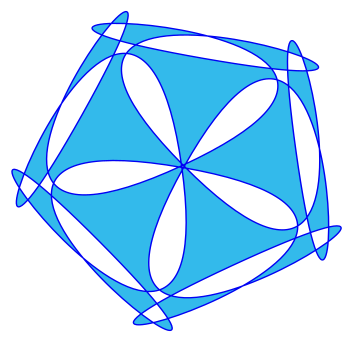
\includegraphics[width=\linewidth]{abstract1}
        % The \linewidth means that it must resize the image to match however big we've specified the subfigure to be!
        \caption{This is my first image.}
        \label{fig:abstract1}
    \end{subfigure}
    \quad\quad % We use quad to add space between the images
    \begin{subfigure}[b]{0.4\columnwidth}
        \centering
        
\includegraphics[width=\linewidth]{abstract2}
        \caption{This is my second image.}
        \label{fig:abstract2}
    \end{subfigure}
    \caption{Two of my finest works of art.}
    \label{fig:abstract_art_subfigure}
\end{figure}

\noindent The code for a subfigure is very similar to a normal figure:
\begin{lstlisting}[style=customtex]
\begin{figure}[h!]
    \centering
    \begin{subfigure}[b]{0.4\columnwidth}
        \centering
        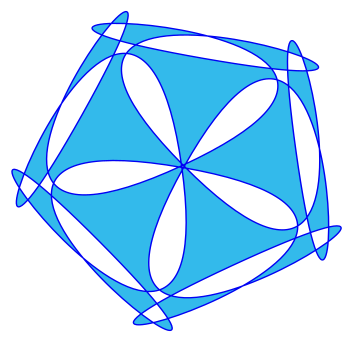
\includegraphics[width=\linewidth]{abstract1}
        \caption{This is my first image.}
        \label{fig:abstract1}
    \end{subfigure}
    \quad\quad
    \begin{subfigure}[b]{0.4\columnwidth}
        \centering
        
\includegraphics[width=\linewidth]{abstract2}
        \caption{This is my second image.}
        \label{fig:abstract2}
    \end{subfigure}
    \caption{Two of my finest works of art.}
    \label{fig:abstract_art_subfigure}
\end{figure}
\end{lstlisting}

\subsection{Labelling and Referencing Figures}
Figures, tables and sections can be referenced at any point in your report as long as you assign it a label. Labels are assigned within the environment, for figures:
\begin{lstlisting}[style=customtex]
\begin{figure}[h]
  % Your figure
  \label{fig:myFigure}
\end{figure}
\end{lstlisting}
\noindent For tables:
\begin{lstlisting}[style=customtex]
\begin{table}[h]
\label{tab:myTable}
  % Your table
\end{table}
\end{lstlisting}
\noindent And for sections:
\begin{lstlisting}[style=customtex]
\section{mySection}
\label{sec:mySection}
\end{lstlisting}

\noindent Now when you'd like to reference these you'd use the ref command:
\begin{lstlisting}[style=customtex]
As shown in Figure~\ref{fig:myFigure}.
As shown in Table~\ref{tab:myTable}.
Explained in Section~\ref{sec:mySection}
\end{lstlisting}

\subsection{Using Cleveref}
\label{sec:cleveref}
Cleveref automatically determines the type of object you're referencing. Instead of using the \textbackslash ref command you'd use the \textbackslash cref command. Now it will not only fill in the figure number but it'll also fill in the type such as table, figure, section, or equation. If you'd like the type to be capitalized (Table vs table) you use \textbackslash Cref.\\

\noindent The following references to figures are using Cleveref: \Cref{tab:measurements_booktabs}, \Cref{fig:abstract_art_subfigure}, \Cref{sec:cleveref}, \Cref{eq:equationtag}, \Cref{fig:abstract1}. Check the difference between these two references: \Cref{tab:measurements_booktabs} vs \cref{tab:measurements_booktabs}.

\begin{lstlisting}[style=customtex]
\Cref{tab:measurements_booktabs} vs \cref{tab:measurements_booktabs}.
\end{lstlisting}

\subsection{Non-Breaking Space}
\noindent In the previous section you may have noticed the $\sim$ sign before the \textbackslash ref. The $\sim$ character ensures that the text before and after it remains on the same line. You'll need to use this OFTEN! Especially when it comes to naming figures, tables, sections, and authors. For instance, I'll use it when I write Kerren~Ortlepp to ensure that ``Kerren'' and ``Ortlepp'' split over two lines.

\subsection{Footnotes}
If you'd like to add a footnote to your document you use the following code:
\begin{lstlisting}[style=customtex]
\footnote{...}
\end{lstlisting}
You'll now see a small number where you've placed your footnote and the text will be at the bottom of the page\footnote{Don't forget to add a full stop to the footnote, it should be a full sentence.}.

\subsection{Creating Lists - Numbered or Bullets}
To create a list we either use an enumeration or itemize environment. The lists be low are generated using the following code:
\begin{lstlisting}[style=customtex]
\begin{enumerate}
  \item Point 1.
  \item Point 2.
  \item Point 3.
\end{enumerate}
\begin{itemize}
  \itemsep0em
  \item Point 1.
  \item Point 2.
  \item Point 3.
\end{itemize}
\end{lstlisting}
\begin{enumerate}
  \item Point 1.
  \item Point 2.
  \item Point 3.
\end{enumerate}
\begin{itemize}
  \itemsep0em
  \item Point 1.
  \item Point 2.
  \item Point 3.
\end{itemize}

\noindent The ``\textbackslash itemsep0em'' removes the additional spacing between each point in the list.

\subsection{Single Column Abstract on a Double Column Document}
In some cases you may want your abstract to go over both columns instead of being in the double column format. To do this you use the following code:

\begin{lstlisting}[style=customtex]
\begin{document}
\twocolumn[
\begin{@twocolumnfalse}
    \maketitle
    \vspace{-1cm} % Reduces the space between the title and the abstract.
    \begin{abstract}
        \noindent Write your abstract here!
    \end{abstract}
\end{@twocolumnfalse}]
\end{lstlisting}

\subsection{Page Size and Margins}
The margins and page size can be modified using the ``geometry'' package. The code is added to the preamble\footnote{The preamble is the code that exists before the \textbackslash begin\{document\}.} and would look something like this:
\begin{lstlisting}[style=customtex]
\geometry{
    a4paper,
    total={170mm,250mm},
    left=25mm,
    right=25mm,
    top=22mm,
    bottom=35mm,
    columnsep=8mm,
    textwidth=172mm
}
\end{lstlisting}
\noindent Please refer to the Blue Book \cite{blue_book} to find the margins and font sizes that should be used in your reports.


\subsection{Verbatim Mode and Listings}
Verbatim mode writes out everything you type to screen. It doesn't see any characters as ``special''. For instance, if you're in verbatim mode and you type the \$ character, it'll output the character as opposed to going into math mode.\\

\noindent In most cases you'd need verbatim mode for writing out code or some form of syntax that uses a lot of special characters. However, there's a better package to use for that known as ``listings''. This is the same package that has been used to show the \LaTeX\ code in previous examples. Verbatim mode would look as follows:\\

\begin{spverbatim}
This is verbatim text       it doesn't ignore spaces or special characters like:
!@#$ $%^&*()-_+`'\|/<>
Often we need these characters when showing some form of syntax. We use listings for that instead of verbatim mode because it offers a lot more functionality!
\end{spverbatim}

\subsection{Vertical and Horizontal Spacing}
Sometimes you need to create some whitespace between objects and text. You can use the \textbackslash vspace and \textbackslash hspace commands which allow you to add vertical and horizontal space respectively. Take a look at the code below and what it produces:\\

\begin{lstlisting}[style=customtex]
\noindent This sentence has a 2cm gap between it and the next sentence.

\vspace{2cm}

\noindent The next sentence.
\end{lstlisting}

\vspace{0.3cm}

\noindent This sentence has a 2cm gap between it and the next sentence.

\vspace{2cm}

\noindent The next sentence.\\

\noindent It's important to note the empty line before and after the \textbackslash vspace command. This has to be there otherwise it doesn't add the vertical space!


\subsection{Section Numbering}
Sometimes we don't want to number a section heading, for instance, if we want an acknowledgement section. In that case we use the ``*'' character when creating the environment and it doesn't give the section a number:
\begin{lstlisting}[style=customtex]
\section*{Acknowledgements}
\end{lstlisting}
Would give the following:
\section*{Acknowledgements}
This section is created to look the same as others but it doesn't add to the section count!



\section{Bibliographies}
Referencing in \LaTeX\ is extremely easy! Using software that creates a Bibtex file (such as JabRef) you can easily create a reference list. To insert the references, at the end of the document you add:
\begin{lstlisting}[style=customtex]
\bibliographystyle{unsrt}
\bibliography{myReferences.bib}
\end{lstlisting}

\noindent Now whenever you need to cite someone (or a number of people) in your text you just use:
\begin{lstlisting}[style=customtex]
Blah blah blah \cite{ref1}.
Blah blah blah \cite{ref1,ref2,ref3}
\end{lstlisting}

\noindent Where ref1, ref2 and ref3 are the unique identifiers that you give to each reference (you'll understand what I mean when you open JabRef).




\section{\tkz Pictures}
\tkz creates high quality images directly in your document! It's similar to a vector based system where you specify the co-ordinates of points and draw lines between them. I'll leave it up to you to read all of the documentation but Figure~\ref{fig:plot} demonstrates the quality of a \tkz image.\\

\begin{figure}[ht!]
  \begin{center}
    \includestandalone[width=0.9\columnwidth]{tikzplot}
  \end{center}
  \caption{My \tkz Plot.}
  \label{fig:plot}
\end{figure}

\noindent In most cases I find it easiest to create a standalone document with your \tkz image:

\begin{lstlisting}[style=customtex]
\documentclass{standalone}
\usepackage{tikz}
\usepackage{amsmath}
\usepackage{pgfplots}

\begin{document}
\begin{tikzpicture}

    % Your Image Goes Here!

\end{tikzpicture}
\end{document}
\end{lstlisting}
\noindent The standalone document allows you to build the file and view it without having to build the whole project. It's not a requirement and does add overhead but it allows you to quickly edit images and view them and import them into your project later!\\

\noindent You then include the image you've just made into your report using:
\begin{lstlisting}[style=customtex]
\begin{figure}[ht!]
  \begin{center}
    \includestandalone[width=0.9\columnwidth]{tikzimagefile}
  \end{center}
  \caption{Caption here}
  \label{fig:myFigure}
\end{figure}
\end{lstlisting}

\noindent This will automatically scale the image for you to fit in the column!

\subsection{\tkz Plotting CSV Files}
Sometimes we need to plot CSV data points directly. Figure~\ref{fig:CSV_figure} demonstrates a plot of a .csv file using \tkz. The axis environment is used and for each plot that should be added the following code is used:
\begin{lstlisting}[style=customtex]
\addplot table [x=x col name, y=y col name, col sep=comma] {file.csv};
\end{lstlisting}

\begin{figure}[ht!]
  \begin{center}
    \includestandalone[width=0.9\columnwidth]{CSVFigure}
  \end{center}
  \caption{Plotting from a CSV.}
  \label{fig:CSV_figure}
\end{figure}

\noindent Take a look at \url{http://pgfplots.sourceforge.net/gallery.html} for more examples of plots of co-ordinates and check out \url{http://pgfplots.sourceforge.net/pgfplots.pdf} for the full documentation. Check out the Section titled ``Markers, Linestyles, (Background-) Colors and Colormaps'' for useful information that you'll often use in your plots. Figure~\ref{fig:CSV_scatter} demonstrates the use of different markers (squares and triangles) in a scatter plot.

\begin{figure}[ht!]
  \begin{center}
    \includestandalone[width=0.9\columnwidth]{Scatter}
  \end{center}
  \caption{Scatter Plot from a CSV.}
  \label{fig:CSV_scatter}
\end{figure}


\noindent On thing to keep in mind is that you're using figures to portray information to the reader. If you can show more information in a single plot you should! Figure~\ref{fig:multiple_axes} demonstrates how you can show more information in a single plot by using two axes instead of one.

\begin{figure}[ht!]
  \begin{center}
    \includestandalone[width=0.9\columnwidth]{MultipleAxes}
  \end{center}
  \caption{Multiple Axes to Show More Information in a Single Plot.}
  \label{fig:multiple_axes}
\end{figure}

\subsection{\tkz Circuits}
You can also create full circuits in \tkz by using the following package:
\begin{lstlisting}[style=customtex]
\usepackage[siunitx]{circuitikz}
\end{lstlisting}

\noindent Now you can create a standalone document with the following structure:
\begin{lstlisting}[style=customtex]
\documentclass{standalone}
\usepackage{tikz}
\usepackage{amsmath}
\usepackage{pgfplots}
\usepackage[siunitx]{circuitikz}

\begin{document}
\begin{circuitikz}

\end{circuitikz}
\end{document}
\end{lstlisting}

\noindent Again you get a high quality circuit output as demonstrated in Figure~\ref{fig:circuit_diagram}. The circuit components are all defined in the document at \url{http://texdoc.net/texmf-dist/doc/latex/circuitikz/circuitikzmanual.pdf}.

\begin{figure}[ht!]
  \begin{center}
    \includestandalone[width=0.9\columnwidth]{circuit}
  \end{center}
  \caption{My \tkz Circuit.}
  \label{fig:circuit_diagram}
\end{figure}


\subsection{\tkz Flow Diagrams}
As an engineering student you WILL need flow diagrams! Check out Figure~\ref{fig:flow_diagram} below. \tkz provides a great way to create flow diagrams in your document. The \tkz code still needs some work in terms of shaping and positioning of blocks but it's easy to move them around.
\begin{figure}[ht!]
  \begin{center}
    \includestandalone[width=0.9\columnwidth]{FlowDiagram}
  \end{center}
  \caption{My \tkz Flow Diagram.}
  \label{fig:flow_diagram}
\end{figure}


\subsection{\tkz 3D Models}
\tkz also supports 3D models, in order to use the 3D functionality you just need to write your co-ordinates in the form $(x,y,z)$. The output is a 2D view of your 3D model, as demonstrated in Figure~\ref{fig:3DModel} below\footnote{Thanks to Harish Vallabhapurapu for the code and permission to use it!}. Check out this URL \url{http://tex.stackexchange.com/questions/42812/3d-bodies-in-tikz} to see how to plot spheres, cones, cubes, and more.\\

\begin{figure}[hb!]
  \begin{center}
    \includestandalone[width=0.9\columnwidth]{3DImage}
  \end{center}
  \caption{An Example of a \tkz 3D Model.}
  \label{fig:3DModel}
\end{figure}



\section{Creating New Commands}
\LaTeX\ allows you to create your own commands. This allows you to adhere to the ``Do Not Repeat Yourself'' (DRY) principle. For instance, if you always add figures in the same way, you could create a command that takes care of most of the information for you.\\

\tikzimage{0.8}{circuit}{This Image has Been Imported in a Single Line!}

\noindent The code that creates Figure~\ref{fig:circuit} image is as follows:
\begin{lstlisting}[style=customtex]
\tikzimage{0.8}{circuit}{This Image has Been Imported in a Single Line!}
\end{lstlisting}
\noindent I'm able to do this because I created a command in the following way:
\begin{lstlisting}[style=customtex]
\newcommand{\tikzimage}[3]{
    \begin{figure}[h!]
        \centering
        \includestandalone[width=.#1\linewidth]{#2}
        \caption[#3]{#3}
        \label{fig:#2}
    \end{figure}
}
\end{lstlisting}
\noindent This is a pretty advanced step and if you're interested in learning how to do it properly, check out the following link, \url{https://www.sharelatex.com/learn/Commands}.

\section{Conclusion}
You have now seen both the basic and advanced aspects of \LaTeX. But seeing is not enough! The only way you'll learn how to use \LaTeX\ is through practical applications, running into errors and troubleshooting them. One thing that you should always remember is that \textbf{GOOGLE IS YOUR FRIEND}. Troubleshooting \LaTeX\ on your own definitely improves your problem solving abilities as an Engineer. So don't just ask people for help when you're struggling - first try to solve the error yourself.


% \bibliographystyle{IEEEtran}
% \bibliography{references}

\printbibliography

\section*{License}
Learning LaTeX is licensed under a Creative Commons Attribution-NonCommercial-ShareAlike 4.0 International License.\\

\noindent You should have received a copy of the license along with this work. If not, see \url{http://creativecommons.org/licenses/by-nc-sa/4.0/}.
\appendix

\section{Extra Stuff to Look Up}
If you're still interested in learning \LaTeX\ I'd suggest you find you about a few more things:
\begin{itemize}
  \item Alignment in a mathematical equation
  \item Spacing in a mathematical equation
  \item Page numbering
  \item Appendices
  \item TabularX to control the widths of the columns in a table
\end{itemize}

\onecolumn

\section{Tikz Images}

The code that creates the Tikz image in Figure~\ref{fig:plot} is as follows:
\begin{lstlisting}[style=customtex]
\documentclass{standalone}
\usepackage{tikz}
\usepackage{amsmath}
\usepackage{pgfplots}
\usepackage{ifthen}
\ifthenelse{\isundefined{\samplesize}}
{
    \newcommand{\samplesize}{500}
}
{
}

\begin{document}
\begin{tikzpicture}
    %Axes
    \draw[->, thick] (0, 0) -- (15, 0) node[below] {$t$};
    \draw[<->, thick] (0, 5) node[above right] {$F(k) = \sum\limits_{k=0}^{k=\infty}\delta (t-k) f(t)$} -- (0, -2.5);
    \draw[smooth, draw opacity = 0.3,dashed] plot[samples=\samplesize, domain=0:14.8] (\x,{ 7 * exp(-0.3*\x) * sin( 2*pi*2/14.8*\x r)});
    \foreach \i in {0,...,29}{
        \draw[fill, draw opacity = 0.6, ultra thin] (\i/2, 0) -- plot[domain=\i/2:\i/2] (\x,{ 7 * exp(-0.3*\i/2) * sin( 2*pi*2/14.8*\i/2 r)}) circle (1pt);
    };
\end{tikzpicture}
\end{document}
\end{lstlisting}

\noindent The code that creates the Tikz image in Figure~\ref{fig:CSV_figure} is as follows:

\begin{lstlisting}[style=customtex]
\documentclass{standalone}
\usepackage{tikz}
\usepackage{amsmath}
\usepackage{pgfplots}
\usepackage{siunitx}
\usepackage{ifthen}
\ifthenelse{\isundefined{\samplesize}}
{
    \newcommand{\samplesize}{500}
}
{
}

\begin{document}
\pgfmathsetmacro{\newPageScale}{0.8}%
\pgfmathsetmacro{\axiswidth}{21*\newPageScale}%
\pgfmathsetmacro{\axisheight}{14.8*\newPageScale}%
% These macros are used to shape the graph to fit nicely in a report.
\begin{tikzpicture}
    \pgfplotsset{ every non boxed x axis/.append style={x axis line style=->} }%
    \pgfplotsset{ every non boxed y axis/.append style={y axis line style=<->, thick} }%
    \begin{axis}[
        width=\axiswidth*1cm, height=\axisheight*1cm,%
        axis y line=left,%
        axis x line=middle,%
        xlabel=\Large{Time (s)},%
        ylabel=\Large{Voltage (V)},%
        xmax = 2.8,
        enlarge y limits=0.05,%
        x label style ={%
            %at={(axis description cs:0,-0.01)},%
            anchor=south%
        },%
        y label style={%
            at={(axis description cs:-0.01,.5)}%,%
        },%
        legend style={%
            anchor= south east%
        },%
        grid style={dashed,black!20},%
        grid = both%
        ]%
        \addplot[mark=.,red!80,thick,smooth] table [x=t, y=v, col sep=comma] {plot.csv};
        \addplot[mark=.,blue!80,thick,smooth] table [x=t, y=v, col sep=comma] {plot2.csv};
        \legend{Input Voltage, Output Voltage};
    \end{axis}
\end{tikzpicture}
\end{document}
\end{lstlisting}
\noindent The code that creates the scatter plot in Figure~\ref{fig:CSV_scatter} is as follows:
\begin{lstlisting}[style=customtex]
\documentclass{standalone}
\usepackage{tikz}
\usepackage{amsmath}
\usepackage{pgfplots}
\usepackage{siunitx}
\usepackage{ifthen}
\ifthenelse{\isundefined{\samplesize}}
{
    \newcommand{\samplesize}{500}
}
{
}

\begin{document}
\pgfmathsetmacro{\newPageScale}{0.8}%
\pgfmathsetmacro{\axiswidth}{21*\newPageScale}%
\pgfmathsetmacro{\axisheight}{14.8*\newPageScale}%
% These macros are used to shape the graph to fit nicely in a report.
\begin{tikzpicture}
    \pgfplotsset{ every non boxed x axis/.append style={x axis line style=->} }%
    \pgfplotsset{ every non boxed y axis/.append style={y axis line style=<->, thick} }%
    \begin{axis}[
        width=\axiswidth*1cm, height=\axisheight*1cm,%
        axis y line=left,%
        axis x line=middle,%
        xlabel=\Large{Time (s)},%
        ylabel=\Large{Voltage (V)},%
        xmax = 1.05,
        enlarge y limits=0.05,%
        x label style ={%
            %at={(axis description cs:0,-0.01)},%
            anchor=south%
        },%
        y label style={%
            at={(axis description cs:-0.01,.5)}%,%
        },%
        legend style={%
            anchor= south east%
        },%
        grid style={dashed,black!20},%
        grid = both%
        ]%
        \addplot[only marks,mark=square,scale=0.1,cyan] table [x=t, y=inenergy, col sep=comma] {scatter.csv};
        \addplot[only marks,mark=o,scale=0.1,violet] table [x=t, y=induceden, col sep=comma] {scatter.csv};
        \legend{Measured Output Energy, Measured Induced Energy};
    \end{axis}
\end{tikzpicture}
\end{document}
\end{lstlisting}

\noindent The code that creates a multi-axis plot in Figure~\ref{fig:multiple_axes} is as follows:
\begin{lstlisting}[style = customtex]
\documentclass{standalone}
\usepackage{tikz}
\usepackage{amsmath}
\usepackage{pgfplots}
\usepackage{siunitx}
\usepackage{ifthen}
\ifthenelse{\isundefined{\samplesize}}
{
    \newcommand{\samplesize}{500}
}
{
}

\begin{document}
\pgfmathsetmacro{\newPageScale}{0.8}%
\pgfmathsetmacro{\axiswidth}{21*\newPageScale}%
\pgfmathsetmacro{\axisheight}{14.8*\newPageScale}%
% These macros are used to shape the graph to fit nicely in a report.
\begin{tikzpicture}
    \pgfplotsset{ every non boxed x axis/.append style={x axis line style=->} }%
    \pgfplotsset{ every non boxed y axis/.append style={y axis line style=<->, thick} }%
    \pgfplotsset{set layers}
    \begin{axis}[
        scale only axis,
        width=\axiswidth*1cm, height=\axisheight*1cm,%
        axis y line=left,%
        axis x line*=middle,%
        xlabel=\Large{Time (s)},%
        ylabel=\Large{Voltage (V)},%
        xmax = 0.5, xmin = 0,
        enlarge y limits=0.05,%
        x label style ={%
            at={(axis description cs:0.5,0.48)},%
            anchor=north east%
        },%
        y label style={%
            at={(axis description cs:-0.01,.5)}%,%
        },%
        legend style={%
            anchor= south east%
        },%
        grid style={dashed,black!20},%
        grid = both%
        ]%
        \addplot[mark=.,scale=0.05,orange,smooth,densely dashed, thick] table [x=t, y=input, col sep=comma] {2Axes.csv}; \label{plot_voltage}
    \end{axis}
    \begin{axis}[
        scale only axis,
        width=\axiswidth*1cm, height=\axisheight*1cm,%
        axis y line=right,%
        axis x line=none,%
        xlabel=\Large{Time (s)},%
        ylabel=\Large{Current (A)},%
        xmax = 0.5, xmin = 0,
        enlarge y limits=0.05,%
        x label style ={%
            anchor=south%
        },%
        y label style={%
            at={(axis description cs:1.01,.4)},%
            anchor=north west
        },%
        legend style={%
            anchor= north east%
        },%
        grid style={dashed,black!20},%
        grid = both%
        ]%
        \addlegendimage{/pgfplots/refstyle=plot_voltage}\addlegendentry{Input Voltage}
        \addplot[mark=.,scale=0.05,darkgray,smooth,thin] table [x=t, y=output, col sep=comma] {2Axes.csv}; \label{plot_current}
        \addlegendentry{Output Current}
    \end{axis}
\end{tikzpicture}
\end{document}
\end{lstlisting}

\noindent The code that creates the Tikz image in Figure~\ref{fig:circuit_diagram} is as follows:
\begin{lstlisting}[style=customtex]
\documentclass{standalone}
\usepackage{tikz}
\usepackage{amsmath}
\usepackage{pgfplots}
\usepackage[siunitx]{circuitikz}

\usepackage{ifthen}
\ifthenelse{\isundefined{\samplesize}}
{
    \newcommand{\samplesize}{500}
}
{
}

\begin{document}
\begin{circuitikz}[ american voltages]
\draw
    (0, 0) to[V=$V_{in}(t)$] (0, 2.5)
    to[sV=$V_n(t)$] (0, 5)
    to[R, l=1<\kilo\ohm> ] (2.5, 5)
    to[L, l=2<\milli\henry>] (5, 5)
    to[C, l=10<\micro\farad>] (5, 0) -- (0, 0);
    \draw (2.5, 0) node[ground] {};
    \draw[dashed, draw opacity=0.4] (2.8, 5.7) -- (6.5, 5.7) -- (6.5, -0.1) -- ( 2.8, -0.1 ) -- cycle;
    \draw (5, 5) -- (7.5, 5) node[circ,] {};
    \draw (5, 0) -- (7.5, 0) node[circ,] {};
    \draw (7.5, 5) node[anchor=north] {$+$};
    \draw (7.5, 0) node[anchor=south] {$-$};
    \draw (7.5, 2.5) node {$V_o(t)$};
    \draw (5-0.2,5.7) node[anchor=south] {Low Pass Filter};
\end{circuitikz}
\end{document}
\end{lstlisting}
\noindent The code that creates the flow diagram in Figure~\ref{fig:flow_diagram} is as follows:

\begin{lstlisting}[style=customtex]
\documentclass{standalone}
\usepackage{tikz}
\usepackage{amsmath}
\usepackage{pgfplots}
\usepackage{siunitx}
\usepackage{xcolor}

\usepackage{ifthen}
\ifthenelse{\isundefined{\samplesize}}
{
    \newcommand{\samplesize}{500}
}
{
}

% Check out https://www.sharelatex.com/blog/2013/08/29/tikz-series-pt3.html for details on the flow diagram building blocks!
\definecolor{decisionColour}{HTML}{B2D1E5}
\definecolor{processColour}{HTML}{E9F2F9}
\definecolor{extraNodeColour}{HTML}{6FB7E9}
\usetikzlibrary{shapes.geometric, arrows}
\tikzstyle{start} = [circle, minimum width=0.5cm, minimum height=0.5cm,text centered, draw=black, fill=black!100, yshift=-0.3cm]
\tikzstyle{end} = [circle, minimum width=0.5cm, minimum height=0.5cm,text centered, draw=black, fill=black!0, yshift=-0.3cm, ultra thick]
\tikzstyle{process} = [rectangle, minimum width=3cm, minimum height=1cm, text centered, draw=black, fill=processColour, rounded corners=0.1cm]
\tikzstyle{decision} = [diamond, text badly centered, draw=black, fill=decisionColour, text width = 3cm]
\tikzstyle{extraNode} = [diamond, minimum width=0.25cm, minimum height=0.25cm, text centered, draw=black, fill=extraNodeColour]
\tikzstyle{arrow} = [thick,->,>=stealth]

\begin{document}%
\begin{tikzpicture}
    \node (start) [start] {} node[anchor=south] {Start};
    \node (procInput) [process, below of = start, yshift=-0.3cm] {Get $x$ from the user};
    % Change the text width and minimum height to get it to look good, it's best to keep them the same so that the decision block is symmetric!
    \node (if1) [decision, below of = procInput, text width = 1.1cm, minimum height = 1.1cm, yshift=-1.2cm] {Is\\ $x \geq 0$?};
    \node (procXGreater)  [process, left of = if1, yshift=-2.3cm, xshift=-1.5cm, text width = 3.5cm] {Print $\sqrt{x}$ to console};
    \node (procXLower)  [process, right of = if1, yshift=-2.3cm, xshift=1.5cm, text width = 3.5cm] {Throw exception:\\Square root of negative};
    \node (finalNode) [extraNode, below of = if1, yshift = -3cm] {};
    \node (end) [end, below of = finalNode] {};
    \draw (end) node[anchor=north, yshift=-0.3cm] {End};
    \draw [arrow] (start) -- (procInput);
    \draw [arrow] (procInput) -- (if1);
    \draw [arrow] (if1) -| node[anchor=south east] {[Yes]} (procXGreater);
    % The -| means horizontal then vertical line
    % That means that |- would draw a vertical line first and then a horizontal. Change them around to see what they do!
    \draw [arrow] (if1) -| node[anchor=south west] {[No]} (procXLower);
    \draw [arrow] (procXGreater) |- (finalNode);
    \draw [arrow] (procXLower) |- (finalNode);
    \draw [arrow] (finalNode) -- (end);
\end{tikzpicture}
\end{document}
\end{lstlisting}

\noindent The code that creates the 3D Tikz image in Figure~\ref{fig:3DModel} is as follows:
\begin{lstlisting}[style=customtex]
\documentclass{standalone}
\usepackage{tikz}
\usepackage{amsmath}
\usepackage{pgfplots}
\usepackage{ifthen}
\ifthenelse{\isundefined{\samplesize}}
{
    \newcommand{\samplesize}{500}
}
{
}
\begin{document}
\begin{tikzpicture}
    \draw[thick,->] (0,0,0) -- (6,0,0) node[anchor=north east]{$x$};
    \draw[thick,->] (0,0,0) -- (0,6,0) node[anchor=north west]{$y$};
    \draw[thick,->] (0,0,0) -- (0,0,6) node[anchor=north west]{$z$};
    \draw[fill, draw opacity = 0.3] (0,0,0) -- (5,5,3) circle (2pt);
    \draw[dashed, draw opacity = 0.2] (5,5,3) -- (5,0,3);
    \draw[dashed, draw opacity = 0.2] (5,5,3) -- (0,5,3);
    \draw[dashed, draw opacity = 0.2] (5,5,3) -- (5,5,0);
    \draw[dashed, draw opacity = 0.2] (5,0,3) -- (5,0,0);
    \draw[dashed, draw opacity = 0.2] (5,0,3) -- (0,0,3);
    \draw[dashed, draw opacity = 0.2] (0,5,3) -- (0,5,0);
    \draw[dashed, draw opacity = 0.2] (0,5,3) -- (0,0,3);
    \draw[dashed, draw opacity = 0.2] (5,5,0) -- (5,0,0);
    \draw[dashed, draw opacity = 0.2] (5,5,0) -- (0,5,0);
    \draw[fill] (0,0,3) node[anchor=north west] {$3$} circle (1pt);
    \draw[fill] (0,5,0) node[anchor=west] {$5$} circle (1pt);
    \draw[fill] (5,0,0) node[anchor=north] {$5$} circle (1pt);
\end{tikzpicture}
\end{document}
\end{lstlisting}
\end{document}